\subsection{Accuracy and cost of the auxiliary gauge solve}
\label{app:gauge-solvers}

The auxiliary solve selects the potential representative entering the Rayleigh quotient. Its accuracy depends on the space used to represent the Poisson correction as well as on the precision of the linear algebra. We compare these effects on a fixed 32-network checkpoint obtained after five updates with Fourier projection and a method-of-fundamental-solutions (MFS) boundary correction. All methods use the same smooth Metaball geometry, neural parameters, analytic derivatives, and relative harmonic field, isolating representative selection from learning.

\paragraph{Common assessment.}
Let $A_\theta$ denote the neural vector potential, with raw column $A_j$. Its scalar divergence forcing is $f_j=\diver A_j$, and $\phi_j$ denotes its numerical scalar correction. We define $\epsilon_P$ as the maximum relative Poisson residual over columns $j=1,\ldots,32$; the sums below use unit weights on independent points $x_q$. On 8192 identical independent fluid points, we report
\begin{equation}
\epsilon_P=\max_{j\leq32}
\frac{\left(\sum_q|f_j(x_q)-\Delta\phi_j(x_q)|^2\right)^{1/2}}
{\left(\sum_q|f_j(x_q)|^2\right)^{1/2}}.
\label{eq:gauge-solver-residual}
\end{equation}
The residual measures the fraction of divergence forcing left after the scalar correction, since $\diver(A_j-\nabla\phi_j)=f_j-\Delta\phi_j$. Relative harmonic overlap is measured on a disjoint 110592-node volume rule after the column transform, and tangential trace on 8192 independent points per wall. Columnwise diagnostics characterize gradient correction, harmonic orthogonality, and boundary trace across all 32 modes. Setup, forward, reverse, and assessment times are measured separately on an RTX 4080 SUPER using native CuPy. Forward/reverse measurements use a 4 GiB allocation pool; the R-marked synchronized setup and assessment measurements use a 12 GiB pool with the same complete workload.

\paragraph{Fourier particular solution and boundary correction.}
On an auxiliary box of side $L=1.12$, an exterior continuation agrees with the original neural potential throughout the fluid. Its divergence is sampled on $193^3$ nodes. Let $k\in\mathbb Z^3$ be an integer wavevector ($\mathbb Z$ denotes integers), $\kappa_k=2\pi k/L$ its physical frequency, $x_0$ the box origin, and $\widehat f_k$ the Fourier coefficients of the sampled forcing. The scalar particular solution $\phi_p$ is
\begin{equation}
\phi_p(x)=-\sum_{k\ne0}\frac{\widehat f_k}{|\kappa_k|^2}
e^{\mathrm i\kappa_k\cdot(x-x_0)}
+\widehat f_0\frac{|x-(0.5,0.5,0.5)|^2}{6}.
\end{equation}
The mean term preserves nonzero-mean forcing. The represented Laplacian is the Fourier interpolant $f_N$ with $N=193$ nodes per axis. The independent residual $f_j-f_N$ measures the source representation at this resolution. A Laplace method-of-fundamental-solutions (MFS) correction with 6144 exterior sources and 18432 boundary collocation nodes enforces the zero Dirichlet trace in least squares \citep{fairweather1998method}. This harmonic boundary correction complements the volume particular solution. We separately test the training arithmetic, FP64 fast Fourier transforms (FFTs) on the same FP32 samples, and an FP64 source/FFT path. A reuse control combines repeated source FFTs and accumulates spectral cotangents before the source-grid inverse FFT, keeping the represented operator unchanged.

\paragraph{Smooth weak projection.}
For a scalar test function $v\in H_0^1(\Omega)$, integration by parts gives the same continuous Dirichlet problem in the form
\begin{equation}
\int_\Omega\nabla v\cdot\nabla\phi\,\dd x
=\int_\Omega\nabla v\cdot A_\theta\,\dd x,
\qquad v\in H_0^1(\Omega).
\end{equation}
We use $C^2$ tensor cubic B-splines {\citep{deboor1978splines}} multiplied by the original analytic zero-trace envelope. Let $b_i$ be the enveloped spline basis functions, $\zeta_i$ their coefficients in $\phi_h=\sum_i\zeta_i b_i$, $\zeta=(\zeta_i)$ their coefficient vector, $\mathsf K$ the gradient stiffness matrix, and $r=(r_i)$ the load vector. The discretization is
\begin{equation}
\mathsf K_{ij}=\sum_qw_q\nabla b_i(x_q)\cdot\nabla b_j(x_q),\quad
r_i=\sum_qw_q\nabla b_i(x_q)\cdot A_\theta(x_q),\quad \mathsf K\zeta=r.
\end{equation}
The neural right-hand side and its parameter reverse require potential values rather than divergence derivatives. Basis gradients and Laplacians are analytic, including across spline knots. Resolution-12, -20, and -24 spaces use 32768, 110592, and 262144 fitting quadrature points. {Matrix-free conjugate gradients \citep{hestenes1952methods} apply the weighted gradient Gram operator; a standard two-level construction \citep{briggs2000multigrid} uses cubic refinement prolongation, symmetric smoothing, and a factored coarse solve.} Severely cut supports are removed when their quadrature gradient-energy diagonal is at most $10^{-5}$ of the maximum. The selection and quadrature remain fixed during differentiation. The algebraic solve residual measures convergence within this space, while \doceqref{eq:gauge-solver-residual} measures the resolved neural forcing.

\paragraph{Volume potential with multipole acceleration.}
{The alternative particular solution follows volume-potential methods \citep{malhotra2016volume} and uses the Newton potential of the piecewise-constant source density $f_h$ over the auxiliary box $B$, with $y$ the integration point:}
\begin{equation}
\phi_p(x)=-\frac1{4\pi}\int_B\frac{f_h(y)}{|x-y|}\,\dd y.
\end{equation}
The volume representation uses constant cuboid densities in $B=[-0.02,1.02]^3$, with the same interior forcing and exterior continuation. Near cuboids, including self interactions, are integrated analytically. {Degree-six Cartesian multipole-to-multipole, multipole-to-local, and local-to-local translations follow the fast multipole method (FMM) \citep{greengard1987fast} to evaluate the far field, whose local Taylor polynomials are harmonic.} The same MFS correction enforces the boundary trace. A source-adaptation variant refines coarse cells when a neighboring density difference, normalized by the per-column coarse-source root mean square (RMS) and maximized over the 32 columns, exceeds $0.5$. The sampling map is fixed for the adjoint, and evaluation uses a uniform tree. The fixed sampling map permits consistent differentiation through the adaptive piecewise-constant representation, following the volume-potential construction \citep{malhotra2016volume}.

% Frozen all-32 checkpoint measurements.
\begin{table}[!htb]\centering\footnotesize\setlength{\tabcolsep}{3pt}
\caption{Gauge-solver accuracy and cost at the fixed checkpoint. \docref{Figure}{fig:gauge-solver-ablation} plots the Poisson residual $\epsilon_P$. Harmonic overlap and tangential trace are percentages; all four timing columns are seconds. Size denotes grid size or retained spline degrees of freedom. Setup and assessment are excluded from forward/reverse. Superscript R denotes a synchronized measurement of the complete workload; forward/reverse columns exclude setup and assessment.}
\label{tab:gauge-solver-ablation}

\begin{tabular}{lrrrrrrr}\toprule
Method&Size&Harm.&Wall tan.&Forward&Reverse&Setup&Assess.\\\midrule
Fourier--MFS & $193^3$ & 0.0177 & 0.6904 & 49.07 & 138.60 & $54.57^{\mathrm R}$ & $23.82^{\mathrm R}$\\
Fourier--MFS, reuse & $193^3$ & 0.0177 & 0.6904 & 48.28 & 136.12 & $62.86^{\mathrm R}$ & $23.32^{\mathrm R}$\\
Spline 12 & 3,106 & 0.0181 & 0.0012 & 6.63 & 6.98 & 1.98 & 5.90\\
Spline 20 & 10,648 & 0.0015 & 0.0012 & 15.40 & 16.60 & 4.75 & 5.91\\
Spline 24 + two-level & 17,086 & 0.0036 & 0.0012 & 71.00 & 78.96 & 11.69 & 5.84\\
Volume FMM 32 & $32^3$ & 0.0242 & 4.8727 & 12.15 & 13.43 & 22.99 & 61.76\\
Volume FMM 64 & $64^3$ & 0.0261 & 3.6399 & 14.23 & 17.66 & 22.82 & 60.63\\
Volume FMM 64 adaptive & $64^3$ & 0.0261 & 3.6399 & 14.53 & 17.96 & 23.71 & 60.51\\\bottomrule\end{tabular}\end{table}

Forward and reverse totals include synchronized component measurements; one-time setup and independent assessment are separate columns. Setup combines spline space/quadrature and optional multigrid construction, or the FMM and fixed harmonic moments; assessment combines independent residual, harmonic, and wall checks. Spline forward timing includes query-point construction. The Fourier and Fourier-reuse measurements share identical neural passes and include source-array export, while spline and volume methods use in-memory sources. Both particular-solution families reuse the geometry-dependent MFS factors.

\begin{table}[!htb]
\centering\small
\caption{Floating-point precision on the same $193^3$ grid. The first two rows use identical source samples. Source time measures one all-32 forward pass, including export.}
\label{tab:gauge-precision}
\begin{tabular}{lrr}\toprule
Arithmetic & $\epsilon_P$ (\%) & Source forward (s)\\\midrule
Training arithmetic & 7.989593 & 37.24 \\
FP32 source, FP64 FFT & 7.989595 & 37.24 \\
FP64 source and FFT & 7.989582 & 266.41 \\
\bottomrule\end{tabular}\end{table}
\paragraph{Representation and arithmetic.}
The precision controls yield nearly identical forcing residuals (\docref{Table}{tab:gauge-precision}). With identical source samples, changing FFT precision produces a relative Laplacian difference of $4.20\times10^{-7}$. Source-space resolution therefore provides the effective control over representative selection at this checkpoint.

Transform reuse preserves forward outputs to the reported precision and changes the source cotangent by a relative $2.50\times10^{-12}$. It reduces the three-evaluation Fourier stage from 9.91 to 8.99 seconds and the source-grid transpose from 12.96 to 10.48 seconds. Total component time decreases from 187.67 to 184.40 seconds (1.74\%); neural source evaluation and parameter differentiation account for 85.5\% of the original total.

\paragraph{Auxiliary-space resolution.}
Refinement systematically improves the spline and volume corrections (\docref{Figure}{fig:gauge-solver-ablation}), while the harmonic projection maintains small overlap across the solver family (\docref{Table}{tab:gauge-solver-ablation}). These complementary diagnostics identify two controls for representative selection: the approximation space resolves gradient content, and the mass projection selects harmonic coordinates. Source adaptation refines 31,432 of 32,768 coarse cells (95.9\%), with 284,224 source evaluations including the coarse pass, compared with 262,144 for the uniform rule. This distribution favors uniform refinement for the present forcing.
\paragraph{Operator consistency.}
FMM evaluation and transpose consistency are tested using $16^3$ cuboids, 48 query points, and two random right-hand sides. The analytic cuboid kernel agrees with nonsingular Gauss integration to relative $7.30\times10^{-11}$. Against direct cuboid integration, increasing the far expansion degree from four to six reduces relative gradient error from $1.38\times10^{-3}$ to $1.90\times10^{-4}$; the degree-six transpose discrepancy is $2.73\times10^{-16}$. These comparisons isolate evaluation of the chosen density from density approximation. For the manufactured scalar $e(x)[1+0.2\sin(2\pi x_1)+0.1x_2x_3]$, the refined spline method gives relative gradient and Poisson errors of $2.85\times10^{-4}$ and $8.82\times10^{-4}$, with linear residual $4.95\times10^{-9}$. Together with \docref{Figure}{fig:gauge-solver-ablation} and \docref{Table}{tab:gauge-solver-ablation}, these checks connect accurate operator evaluation to systematic control through auxiliary-space refinement.

\begin{figure}[!htb]
\centering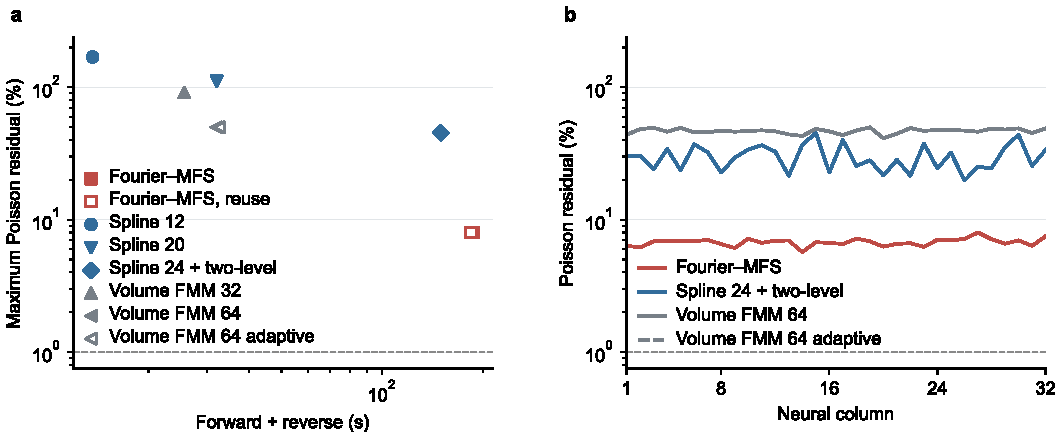
\includegraphics[width=\linewidth,height=.72\textheight,keepaspectratio]{gauge_solver_ablation.pdf}
\caption{\textbf{Gauge-solver accuracy and cost.} Left: all-32 forward-plus-reverse time versus independent Poisson residual. Right: per-column residuals for Fourier--MFS and the finest tested spline and volume spaces. All methods evaluate the same fixed neural checkpoint.}
\label{fig:gauge-solver-ablation}
\end{figure}


\paragraph{Connection to the velocity span.}
At a fixed network, each scalar correction has zero curl, so all solvers retain the same 32-dimensional analytic velocity span. The solver comparison therefore measures representative selection for the potential objective; changes to the learned velocity span arise through subsequent optimization.
